\makeatletter
\ifx\@nodocument\relax
  % Included from a document that is already running.
  \makeatother
  \providecommand{\toprule}{\hline}
  \providecommand{\midrule}{\hline}
  \providecommand{\bottomrule}{\hline}
  \providecommand{\cmidrule}[2][]{}
  \providecommand{\mynote}[1]{{\color{blue}[#1]}}
  \newcommand{\numericalexperimentsclose}{}
\else
  \makeatother
  \documentclass[11pt]{article}
  \usepackage{graphicx}
  \usepackage{amssymb, amsfonts, amsmath, amsthm}
  \usepackage[margin=1in, footskip=1cm, headheight = 1.5cm]{geometry}
  \usepackage[sort]{natbib}
  \usepackage{booktabs}
  \usepackage{hyperref}
  \hypersetup{colorlinks=true, linkcolor=blue, citecolor=cyan}
  \bibliographystyle{unsrtnat}
  \usepackage[nameinlink]{cleveref}
  % Shared macros and environments for every document in tex/.
% Seeded from the group's standard template; project-specific additions are
% collected at the end.

% Commands
\newcommand{\eg}{{\it e.g.}}
\newcommand{\ie}{{\it i.e.}}

% Sets
\newcommand{\ones}{\mathbf 1}
\newcommand{\reals}{{\mathbf R}}
\newcommand{\integers}{{\mathbf  Z}}
\newcommand{\symm}{{\mathbf S}}  % symmetric matrices
\newcommand{\NPhard}{\mbox{$\mathcal{NP}$-hard}}
\newcommand{\prob}{{\mathbf P}}
\newcommand{\distrib}{{\mathcal P}}
\newcommand{\identity}{I}
\newcommand{\nullspace}{{\mathcal N}}
\newcommand{\range}{{\mathcal R}}
\newcommand{\Rank}{\mathop{\bf rank}}
\newcommand{\Tr}{\mathop{\bf Tr}}
\newcommand{\diag}{\mathop{\bf diag}}
\newcommand{\lambdamax}{{\lambda_{\rm max}}}
\newcommand{\lambdamin}{\lambda_{\rm min}}
\newcommand{\Expect}{{\bf E{}}}
\newcommand{\Co}{{\mathop {\bf Co}}} % convex hull
\newcommand{\dist}{\mathop{\bf dist{}}}
\newcommand{\argmin}{\mathop{\rm argmin}}
\newcommand{\argmax}{\mathop{\rm argmax}}
\newcommand{\epi}{\mathop{\bf epi}} % epigraph
\newcommand{\Vol}{\mathop{\bf vol}}
\newcommand{\dom}{\mathop{\bf dom}} % domain
\newcommand{\intr}{\mathop{\bf int}}

\newcommand{\sign}{\mathop{\bf sign}}
\newcommand{\round}{\mathop{\bf round}}

% Sections (for citation)
\newcommand{\Sec}{Section\;}

% Create theorems and other environments
\newtheorem{theorem}{Theorem}[section]  % Restart counter every section
\newtheorem{lemma}{Lemma}[section]  % Restart counter every section
\newtheorem{corollary}{Corollary}[theorem]  % Restart counter every theorem
\newtheorem{proposition}{Proposition}[section]
\newtheorem{assumption}{Assumption}[section]

\theoremstyle{definition}
\newtheorem{definition}{Definition}[section]
\newtheorem{problem}{Problem}[section]

\theoremstyle{remark}
\newtheorem{example}{Example}[section]
\newtheorem{exercise}{Exercise}[section]
\newtheorem{remark}{Remark}[section]

% lowercase names
\crefname{equation}{}{}
\crefname{assumption}{assumption}{assumptions}
\crefname{algocf}{Algorithm}{Algorithms}

% Acronyms.  Defined only when the preamble loaded the glossaries package, so
% that this file can be \input from a document that does not use acronyms.
\makeatletter
\@ifundefined{newacronym}{}{%
  \newacronym{LP}{LP}{linear program}
  \newacronym{QP}{QP}{quadratic program}
  \newacronym{MIQP}{MIQP}{mixed-integer quadratic program}
  \newacronym{MIP}{MIP}{mixed-integer program}
  \newacronym{MILP}{MILP}{mixed-integer linear program}
  \newacronym{MINLP}{MINLP}{mixed-integer nonlinear program}
  \newacronym{sBB}{sBB}{spatial branch and bound}
  \newacronym{PWA}{PWA}{piecewise affine}
  \newacronym{SVM}{SVM}{support vector machines}
  \newacronym{ReLU}{ReLU}{rectified linear unit}
  \newacronym{CPU}{CPU}{central processing unit}
  \newacronym{GPU}{GPU}{graphics processing unit}
  \newacronym{MPC}{MPC}{model predictive control}
  \newacronym{ADMM}{ADMM}{alternating direction method of multipliers}
  \newacronym{ADP}{ADP}{approximate dynamic programming}
  \newacronym{FPGA}{FPGA}{field-programmable gate array}
  \newacronym{DRS}{DRS}{Douglas--Rachford splitting}
  \newacronym{RandNLA}{RandNLA}{randomized numerical linear algebra}
  \newacronym{CG}{CG}{conjugate gradients}
  \newacronym{GMRES}{GMRES}{generalized minimal residual method}
}
\makeatother

% Project-specific definitions
\newcommand{\prox}{\mathrm{prox}}
\newcommand{\R}{\mathbb{R}}
\newcommand{\Prob}{\mathbb{P}}

% Zero set, graph, and fixed point set of an operator, in the style of \dom.
\newcommand{\zer}{\mathop{\bf zer}}
\newcommand{\gra}{\mathop{\bf gra}}
\newcommand{\fix}{\mathop{\bf fix}}

\newcommand{\Acal}{{A}}
\newcommand{\Bcal}{{B}}
\newcommand{\Ccal}{{C}}
\newcommand{\Fcal}{\mathcal{F}}
\newcommand{\Dcal}{\mathcal{D}}
\newcommand{\Hcal}{\mathcal{H}}
\newcommand{\Mcal}{{M}}
\DeclarePairedDelimiter{\norm}{\lVert}{\rVert}

\DeclarePairedDelimiterX{\ipx}[2]{\langle}{\rangle}{#1,#2}
% \ip{a}{b} sizes its angle brackets with \left and \right; \ip*{a}{b} keeps them fixed.
\makeatletter
\newcommand{\ip}{\@ifstar{\ipx}{\ipx*}}
\makeatother

  \crefname{equation}{}{}
  \newcommand{\mynote}[1]{{\color{blue}[#1]}}
  \newcommand{\numericalexperimentsclose}{\bibliography{bibliography}\end{document}}
  \title{Numerical Results (draft section)}
  \author{Pranav Reddy}
  \date{\today}
  \begin{document}
  \maketitle
\fi

\section{Numerical Experiments}\label{sec:numerical-experiments}
We numerically examine the strength of our conclusions and how well the results hold up to empirical scrutiny.
\TODO{rewrite numerical experiments}
% We first study \DIFdel{the two algorithms listed above: PPM and ADMM}\DIFadd{PPM and the original partially inexact ADMM method described in \Cref{sec:numerical-experiments-admm}}, with the goal of examining how inexactness impacts the performance of these algorithms as well as how conservative the theoretical findings are.
We also include a study of a rotation operator which highlights more adversarial behavior one could encounter.
Here, performance refers both to inner and outer iteration complexity, as well as wall-clock time.
All experiments were run on the author's MacBook Pro (Apple M5 Max, 128 GB of memory) in Python 3.14.5 with NumPy 2.5.3, SciPy 1.18.1, CVXPY 1.9.3, and Clarabel 0.11.1.
The code is available at \url{https://github.com/stellatogrp/rand_nla_fom}.
We declare that the code for these experiments was generated with the assistance of Claude, and we take full responsibility for the content of this section.

\subsection{Inexact Proximal Point}
In this section, we empirically study the algorithm theoretically examined in \Cref{prop:optimal-sigma-gradient-descent-inside-ppm}.
We test \Cref{alg:stopping-time-algorithm} on an instance of linear regression with Huber loss \citep{huber1964huberloss}.
That is,
\begin{equation} \label{eq:huber-loss-problem}
    \begin{array}{ll}
        \text{minimize} & \sum_{i=1}^{m} h_\rho(a_i^\top x - b_i),
    \end{array}
\end{equation}
where $x\in\R^n$ is the optimization variable, $\left\{ (a_i,b_i) \right\}_{i=1}^m$ is the data, and $h_\rho:\R\to\R$ is the Huber loss function with parameter $\rho$:
\begin{align}
    h_\rho(x) = \begin{cases}
        \frac{1}{2}x^2, & |x|\leq \rho, \\
        \rho(|x|-\frac{1}{2}\rho), & |x| \geq \rho.
    \end{cases}
\end{align}
We define the objective $f(x) = \sum_{i=1}^{m} h_\rho(a_i^\top x - b_i)$ to be the sum of the Huber losses of the residuals.
The parameter $\rho$ controls the tradeoff between the $\ell_2$ and $\ell_1$ loss.
We set the parameter $\rho = \frac{1}{2}$, and note that the $L$-smoothness constant of the objective in \Cref{eq:huber-loss-problem} is $L = \norm{A}_2^2$, where $A$ is the design matrix whose rows are $a_i$.
Its gradient can be easily computed in closed form as $\nabla f(x) = A^\top \Pi_{[-\rho,\rho]^m}(Ax-b)$, where $\Pi_{[-\rho,\rho]^m}$ is the projection onto the $m$-box $[-\rho,\rho]^m$.

We construct synthetic data $\left\{ (a_i,b_i) \right\}_{i=1}^m$, with $m = 3000$ and $n = 2000$, where $a_i \sim\mathcal{N}(0,m^{-1}I_n)$ are i.i.d.
We sample $x_{\mathrm{true}}\sim\mathcal{N}(0,I_n)$ and set $b = A x_{\mathrm{true}} + 0.1 \eta$, where $\eta\sim\mathcal{N}(0,I_m)$.
We then select uniformly at random 10\% of the entries of $b$ (300 entries) to be perturbed by a $\mathrm{Uniform}([-8,-3]\cup[3,8])$ disturbance.
We generate 100 sets of problem data and run each configuration of algorithm parameters on these 100 instances.
For a baseline, we compare to the solution time of CVXPY using the Clarabel solver \citep{agrawal2018rewriting,diamond2016cvxpy,goulart2024clarabel}.

The proximal subproblem is to solve
\begin{align}
    \prox_{\gamma f}(x) = \argmin_{y\in\R^n} \quad \sum_{i=1}^{m} h_\rho(a_i^\top y - b_i) + \frac{1}{2\gamma}\norm{y - x}^2, \label{eq:prox-huber}
\end{align}
which has no known closed-form solution.
We use (unaccelerated) gradient descent with fixed stepsize $\gamma_{\mathrm{GD}} = \frac{2\gamma}{\gamma L + 2}$ to solve the proximal subproblem \Cref{eq:prox-huber} with proximal parameter $\gamma = \frac{10}{L}$.
We run the algorithm until the gradient is sufficiently small: $\norm{\nabla f(x_k)} \leq \delta$, and we set $\delta = 10^{-9}$.
Since the solution to Huber regression is not known in closed form, this is a practical convergence metric to use.
We can substitute this setup into \Cref{alg:stopping-time-algorithm} directly, letting $\Ccal = I$ and $\Acal=\nabla f$.
Since this is precisely the scenario of \Cref{prop:optimal-sigma-gradient-descent-inside-ppm}, we compare our empirical results against the theoretical guarantees of the algorithm.

Our main focus is to understand the tradeoff between the work required for a given subproblem and the speed of convergence of the outer method.
In this spirit, we sweep over the parameters $\sigma\in\left\{ 0.01, 0.05, 0.2, 0.5, 0.9, 1 \right\}$ (inexactness) and $s\in\left\{ 1,2,5,10,20 \right\}$ (stride).
The $\sigma$ sweep runs at stride $s = 1$, the stride sweep at $\sigma = 0.1$, and every run starts from $w_0 = 0$.
Since the theory guarantees termination only for $\sigma<1$, every inexact run is also subject to a hard stop: $10^{6}$ inner iterations in total or $300$ seconds of wall-clock time, checked at every relative error test, in addition to a cap of $50{,}000$ outer iterations.
The near-exact baseline solves each subproblem to an inner residual $\gamma\norm{\nabla\varphi_k}$ of $10^{-12}$.
The near-exact baseline always terminates and is subject to the cap on inner iterations only.
No run reported here reached any of these limits, including those at $\sigma=1$.

\Cref{fig:ppm-huber-wall-clock-times} shows a comparison of the shifted geometric mean (SGM) of the wall-clock times for the different choices of parameters.
For this study, choosing the median time or the SGM of the results made no difference in the ordering of configurations.
Reducing subproblem accuracy improves the speed of convergence both in wall-clock time and gradient evaluations, as seen in \Cref{fig:ppm-huber-wall-clock-times,fig:ppm-huber-outer-convergence}, respectively.
In fact, sufficiently inexact iterations outperform running the same gradient descent algorithm on the original problem \Cref{eq:huber-loss-problem} itself.

\begin{figure}
    \centering
    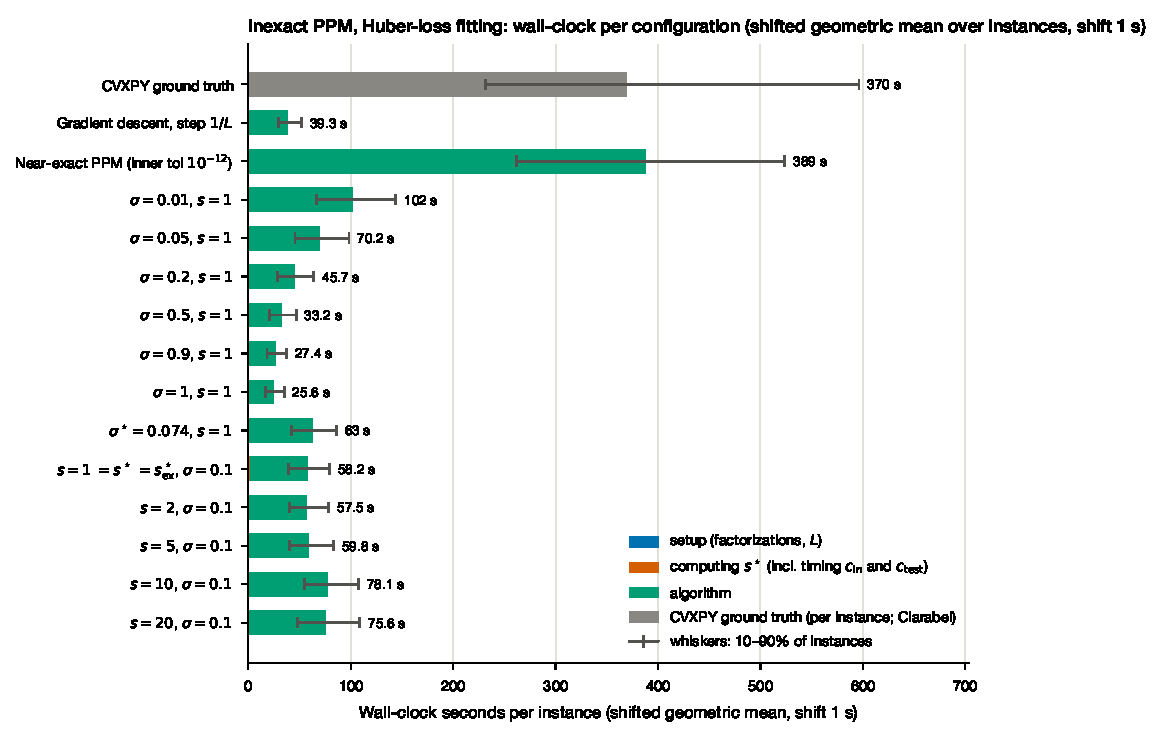
\includegraphics[width=\textwidth]{../results/numerical_experiments/ppm_huber/walltime_sgm.pdf}
    \caption{Wall-clock time per configuration on the Huber instances \Cref{eq:huber-loss-problem} with $n = 2000$ and $m = 3000$: the shifted geometric mean over the 100 instances of the setup time, of the time to compute $s^\star$ where it is used (including the timing of $c_{\mathrm{in}}$ and $c_{\mathrm{test}}$), and of the algorithm time, stacked.
    Computing $\sigma^\star$ needs only $\alpha$ and $C_0$ and takes under a millisecond, so its bar has no such segment.
    Whiskers span the 10th to the 90th percentile of the algorithm time, and the top bar is the CVXPY (Clarabel) solve time for scale.
    The configurations are gradient descent on \Cref{eq:huber-loss-problem}, the near-exact method, the $\sigma$ sweep at $s = 1$ (including $\sigma^\star$), and the $s$ sweep at $\sigma = 0.1$ (including $s^\star$).
    Sufficiently inexact runs are faster than both the near-exact method and gradient descent.}\label{fig:ppm-huber-wall-clock-times}
\end{figure}

\Cref{fig:ppm-huber-outer-convergence} compares the convergence behavior of the configurations; \Cref{fig:ppm-huber-outer-convergence-zoom} in \Cref{sec:additional-ppm} magnifies its outer-iteration panels.
Despite producing virtually identical suboptimality and stationarity residuals, the performance over the \emph{inner} work is different.
In fact, the near-exact PPM performs worse than all other configurations in this regard.
Moreover, the highly inexact choices of parameters, $\sigma=0.5$ and $\sigma=0.9$, outperform vanilla gradient descent in terms of the number of gradient evaluations.
Even $\sigma=0.2$ is competitive with gradient descent.

\begin{figure}
    \centering
    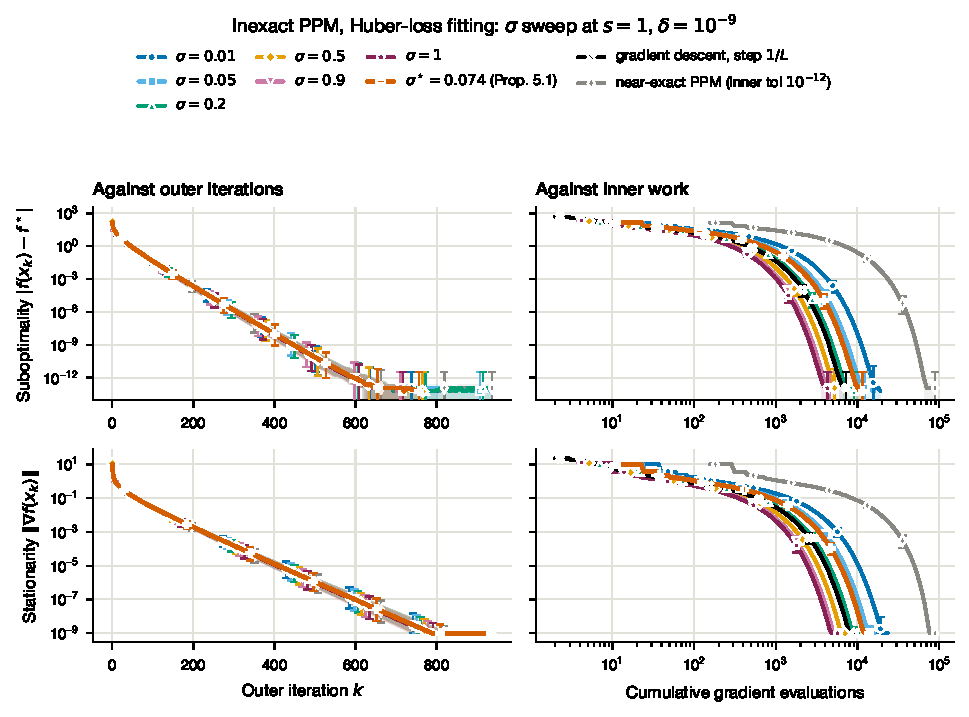
\includegraphics[width=\textwidth]{../results/numerical_experiments/ppm_huber/convergence_sigma.pdf}
    \caption{Convergence of \Cref{alg:stopping-time-algorithm} on the Huber instances \Cref{eq:huber-loss-problem} for the $\sigma$ sweep at $s = 1$, for $\sigma^\star$, and for the near-exact method: suboptimality $|f(x_k) - f^\star|$ (top) and stationarity $\norm{\nabla f(x_k)}$ (bottom) against outer iterations (left) and against cumulative gradient evaluations (right).
    Lines are medians over the 100 instances, bands interquartile ranges, and whiskers the 10th to the 90th percentiles; gradient descent has no outer iterations and appears against gradient evaluations only.
    The curves nearly coincide against outer iterations but separate widely against inner work, where the near-exact method is the slowest.}\label{fig:ppm-huber-outer-convergence}
\end{figure}

The magnified view in \Cref{fig:ppm-huber-outer-convergence-zoom} confirms that the convergence metrics are nearly indistinguishable, suggesting that there is little effect of inexactness on the outer iterations.
The theory predicts a multiplicative factor of $\frac{1+\sigma}{1-\sigma}$ in the worst-case convergence rate, which equals 19 for $\sigma = 0.9$.
This factor is not visible in the numerics, highlighting the pessimism of the theory.

The trajectory of the inexact iterates tends to closely follow that of the near-exact algorithm.
In \Cref{fig:ppm-huber-trajectories}, the near-exact solutions to the subproblems of the inexact PPM (hollow markers) closely match the trajectory of the near-exact PPM (dashed line).
The inexact method required 47 outer iterations ($K_\delta = 47$), but the near-exact method required only 22 ($K_\delta = 22$).
However, the inexact PPM with $\sigma = 0.9$ used only 142 gradient evaluations, whereas the near-exact PPM used 1,571 gradient evaluations, over 10 times the number of gradient evaluations.
\begin{figure}
    \centering
    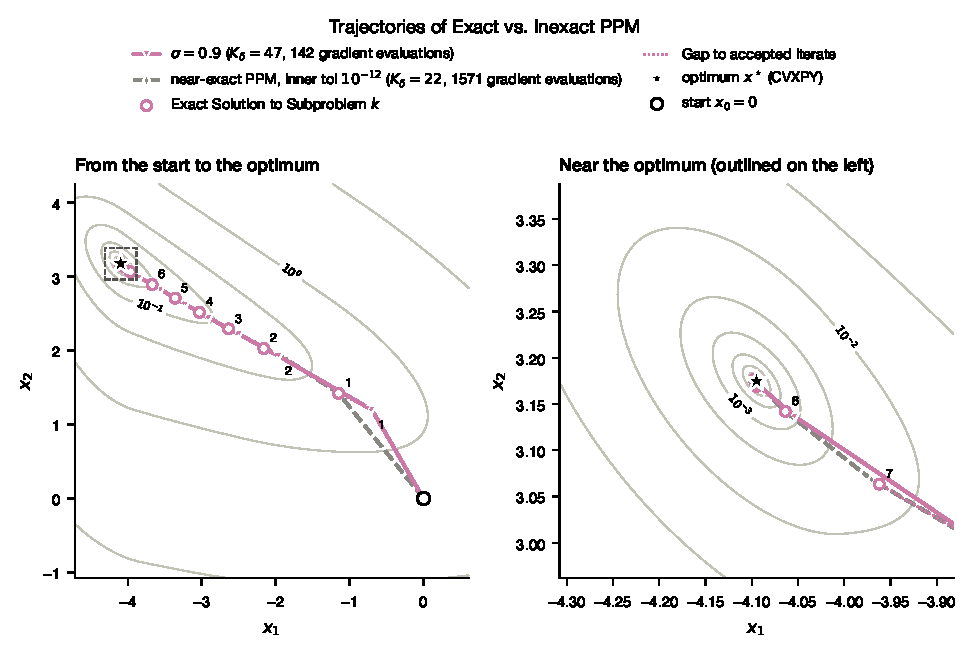
\includegraphics[width=\textwidth]{../results/numerical_experiments/ppm_huber_2d/trajectory_2d_exact.pdf}
    \caption{Accepted iterates of the near-exact method (dashed) and of one inexact run with $\sigma = 0.9$ and $s = 1$ on a two-dimensional Huber instance, over contours of $f - f^\star$: left, from the start $x_0 = 0$ to the optimum; right, the neighborhood of the optimum outlined on the left.
    Hollow markers are the exact solutions $J(w_k)$ of the subproblems that the inexact run approximated, joined to the accepted iterate by dotted segments; a point that passed several consecutive acceptance tests without an inner step carries all their iteration numbers.
    The inexact run takes 47 outer iterations against 22, but 142 gradient evaluations against 1,571.}\label{fig:ppm-huber-trajectories}
\end{figure}

Additionally, we compare the predicted cost of choosing different values of the stride $s$ (lines 4--10 of \Cref{alg:stopping-time-algorithm}).
The relaxed bound refers to that of \Cref{lem:check-frequency-s-star}, while the unrelaxed bound refers to \Cref{rem:b-star-remark}.
The unrelaxed bound gives a tighter bound, but only up to a nearly constant factor.
Moreover, the conservatism of \Cref{lem:check-frequency-s-star} can be seen in \Cref{fig:ppm-huber-optimal-b-star-model}, where increasing the stride does not seem to affect the time per outer iteration significantly.
The cost of checking depends on factors such as hardware types and availability, difficulty of subproblems, implementation details, and so forth, but using the $s^\star$ defined in \Cref{lem:check-frequency-s-star} seems to be a good heuristic.

\begin{figure}
    \centering
    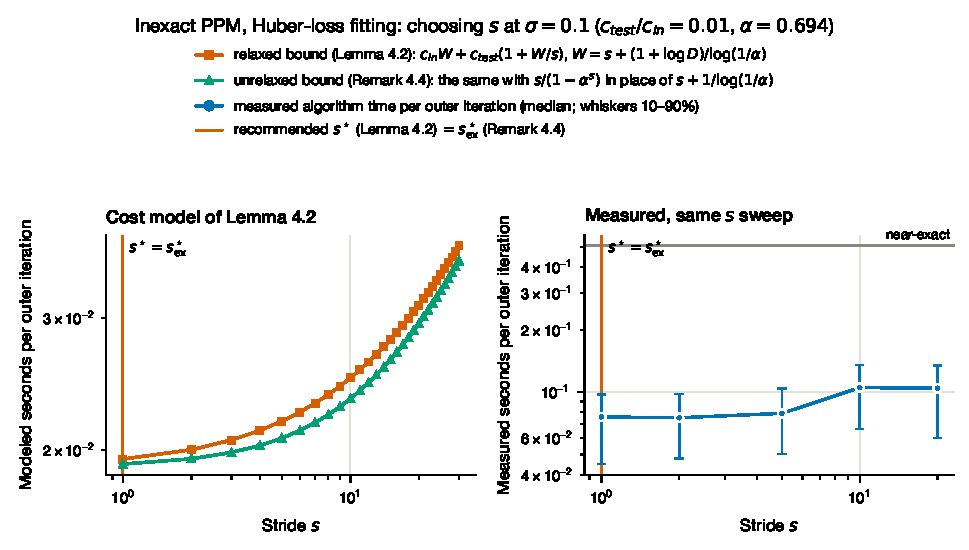
\includegraphics[width=\textwidth]{../results/numerical_experiments/ppm_huber/bstar_model.pdf}
    \caption{Choosing the stride on the Huber instances.
    Left, the modeled seconds per outer iteration as a function of $s$ from \Cref{lem:check-frequency-s-star} (relaxed bound) and from \Cref{rem:b-star-remark} (unrelaxed bound), with their integer minimizers marked; right, the measured seconds per outer iteration of the $s$ sweep at $\sigma = 0.1$ (median over the 100 instances; whiskers from the 10th to the 90th percentile), with the level of the near-exact method as a horizontal line.
    The relaxation shifts the model by a nearly constant factor, and the measured time is almost flat in $s$.}\label{fig:ppm-huber-optimal-b-star-model}
\end{figure}

\subsection{Inexact ADMM}\label{sec:numerical-experiments-admm}
In this section, we empirically study the \DIFdelbegin \DIFdel{performance of \Cref{alg:inexact-admm} }\DIFdelend \DIFaddbegin \DIFadd{partially inexact ADMM method of \citet{EcksteinRelativeError2018} }\DIFaddend on a quadratic program with linear equality constraints\DIFaddbegin \DIFadd{.
These experiments use the consensus splitting $E=I$, no additional proximal term, and an exact $g$-solve at $x_k-\frac{1}{c} a_k $; only the $f$-solve is inexact.
The matrix $A$ below defines the indicator in $g$ and is distinct from the splitting map $E$ in \Cref{eq:admm-problem}}\DIFaddend .
That is,
\begin{equation}\label{eq:admm-qp}
    \begin{array}{ll}
    \text{minimize} & \frac{1}{2}x^\top Q x + d^\top x, \\
    \text{subject to} &Ax = b,
    \end{array}
\end{equation}
where $x\in\R^n$ is the optimization variable and $A\in\R^{m\times n}$, $Q\succ 0$, $d\in\R^n$, and $b\in\R^m$ are the problem data.
We take $m = 600$ and $n = 2000$ in these trials, with penalty $c = \frac{L}{10}$, where $L$ is the smoothness constant of the objective.
Our stopping tolerance is $\delta = 10^{-9}$.
The sweeps are the same as for the Huber instances: the $\sigma$ sweep runs at $s = 1$ and the stride sweep at $\sigma = 0.1$.
Every run starts from $z_0 = p_0 = 0$.
As before, we compare to the solution time of CVXPY using the Clarabel solver, but we also include a closed-form solution for the $x$-subproblem in \Cref{eq:admm-x-subproblem-numerical-experiments-qp}.
Since the optimality conditions for the $x$-subproblem \Cref{eq:admm-x-subproblem-numerical-experiments-qp} are a linear system, $(Q + cI)x = cz_k - d - p_k$, we compare an iterative solution to using a Cholesky factorization of the matrix $Q + cI$.
In large-scale applications, obtaining such a factorization may not be feasible, but this is still implemented in some well-known solvers such as OSQP \citep{osqp-original-paper}.

We sample $Q = V\diag(\lambda)V^\top$, where $\lambda$ is log-spaced in $[\kappa^{-1},1]$, $V$ is the orthogonal factor of the QR decomposition of a matrix with i.i.d.\ $\mathcal{N}(0,1)$ entries, and $\kappa = 10^4$.
This also shows that $\norm{Q}_2 = 1$ is the $L$-smoothness constant of the objective.
The regularized matrix $Q+cI$ appearing in the $x$-subproblem \Cref{eq:admm-x-subproblem-numerical-experiments-qp} has $\kappa_c := \kappa_2(Q + cI) = \frac{1+c}{10^{-4} +c} \leq 1 + \frac{L}{c}$.
We use the estimate $\kappa_c \leq 1 + \frac{L}{c} = 11$ for the estimation of parameters.
In this setup, the exact value is $\kappa_c \approx 10.99$, so this approximation is good for matrices with small eigenvalues.
The constraint matrix $A$ has i.i.d.\ $\mathcal{N}(0, n^{-1})$ entries.
We generate ground truth primal and dual solutions $x^\star\in\R^n$ and $\nu^\star\in\R^m$ with i.i.d.\ $\mathcal{N}(0, n^{-1})$ and $\mathcal{N}(0, m^{-1})$ entries, respectively.
The data $d$ and $b$ are computed such that the pair $(x^\star,\nu^\star)$ solves the Karush--Kuhn--Tucker (KKT) system, so that the ADMM dual $p_k$ converges to $-(Qx^\star + d) = A^\top\nu^\star$.
Since $Q\succ 0$ and $A$ is full rank, the solution is unique.
\DIFdelbegin \DIFdel{The subproblems \Cref{eq:admm-iterates} become
}\DIFdelend \DIFaddbegin \DIFadd{For the partially inexact method used here, let $a_k=Qx_k+d$ and compute the candidates and accepted multiplier update as
}\DIFaddend \begin{subequations}\label{eq:admm-iterates-numerical-experiments-qp}
\DIFdelbegin \begin{align}
    \DIFdel{x_{k} }&\DIFdel{\approx \argmin_{x} \left\{ \frac{1}{2}x^\top Q x + d^\top x + \ip{p_k}{x} + \frac{c}{2}\norm{x-z_k}^2 \right\}, }\\
    \DIFdel{p_{k+1} }&\DIFdel{= p_k + c(x_{k}-z_k), }\\
    \DIFdel{z_{k+1} }&\DIFdel{= \argmin_{z}\left\{  \mathcal{I}_{\left\{ z \mid Az = b \right\}}(z) - \ip{p_{k+1}}{z} + \frac{c}{2}\norm{z-x_{k}}^2 \right\}. %DIFDELCMD < %%%
}\end{align}%DIFAUXCMD
\DIFdelend \DIFaddbegin \begin{align}
    \DIFadd{x_k}&\DIFadd{\approx\argmin_x\left\{\frac{1}{2}x^\top Qx+d^\top x+\ip{p_k}{x}+\frac{c}{2}\norm{x-z_k}^2\right\},\label{eq:admm-x-subproblem-numerical-experiments-qp}}\\
    \DIFadd{z_{k+1}}&\DIFadd{=\argmin_z\left\{\mathcal{I}_{\{z\mid Az=b\}}(z)+\ip{a_k}{z}+\frac{c}{2}\norm{z-x_k}^2\right\},\label{eq:admm-z-subproblem-numerical-experiments-qp}}\\
    \DIFadd{p_{k+1}}&\DIFadd{=p_k+c(x_k-z_k).
}\end{align}\DIFaddend
\end{subequations}
\DIFdelbegin \DIFdel{Substituting this into \Cref{alg:inexact-admm} yields the algorithm found in the code.
Note that the $z$-subproblem \Cref{eq:admm-z-subproblem-numerical-experiments-qp} is the projection of $x_k + \frac{1}{c}p_{k+1}$ (of $x_k - \frac{1}{c} a_k $ in \Cref{alg:inexact-admm}) onto the affine subspace $\{z \mid Az = b\}$}\DIFdelend \DIFaddbegin \DIFadd{At each check, the method first terminates if $\norm{x_k-z_{k+1}}\leq\delta$ and otherwise accepts the multiplier update if
}\begin{align}
    \DIFadd{\norm{a_k+p_k+c(x_k-z_k)}\leq\sigma\norm{a_k+p_k+c(z_{k+1}-z_k)}.
}\end{align}
\DIFadd{For $k\geq1$, the first solve is warm-started at $x_{k-1}$.
If neither test passes, the first solve is refined through $s$ GMRES steps before the next check.
The second subproblem projects $x_k-\frac{1}{c} a_k $ onto $\{z\mid Az=b\}$}\DIFaddend , which can be done to machine precision\DIFaddbegin \DIFadd{.
Its target agrees with $x_k+\frac{1}{c}p_{k+1}$ when the first solve is exact.
Each check uses one such projection, shared by the terminal and relative error tests; this is the test cost $c_{\mathrm{test}}$ in \Cref{lem:check-frequency-s-star}}\DIFaddend .
The inexactness arises from the $x$-subproblem, which we internally solve using GMRES, since the optimality conditions are a positive definite linear system.
We remark that in this setup, $C_0 =4$ and $\sqrt{\alpha} = \frac{\sqrt{\kappa_c}-1}{\sqrt{\kappa_c}+1}$, so $\alpha\approx 0.288$.
The constants come from an application of the Chebyshev bound in the proof of \citet[Theorem 38.5]{Trefethen1997NumericalLinearAlgebra} to \citet[Proposition 4]{saad1986GMRES}.
\begin{admmaddition}


If gradient descent is used instead for the first subproblem of this partially inexact method, $L$-smoothness with $L>0$ and stepsize $2/(L+2c)$ give
\begin{align}
    \alpha=\left(\frac{L}{L+2c}\right)^2,\qquad C_0=\left(1+\frac{L}{c}\right)^2.
\end{align}
Indeed, its graph residual is $c^{-1}\nabla\varphi_k(x)$ for $\varphi_k(x)=f(x)+c\norm{x-w_k}^2/2$, so these constants follow from \Cref{prop:optimal-sigma-gradient-descent-inside-ppm} with proximal parameter $1/c$.
These are constants for the original method with only the first solve inexact; the fully inexact method of \Cref{alg:inexact-admm} requires contraction of its joint residual.
\end{admmaddition}


The wall-clock times in \Cref{fig:admm-qp-wall-clock-times} demonstrate that the theory is fairly conservative.
Very inexact iterations appear to have \emph{better} performance than their exact counterparts.
We attribute this to the ability to move in generally the correct direction, even though the precise step may not be accurate.
However, all configurations using an iterative method to solve the $x$-subproblem in \Cref{eq:admm-x-subproblem-numerical-experiments-qp} are slower than using the Cholesky factorization of $Q + cI$.
We do not consider this to be a limitation, since in many applications such a closed-form solution is either not available or not feasible to implement.

\begin{figure}
    \centering
    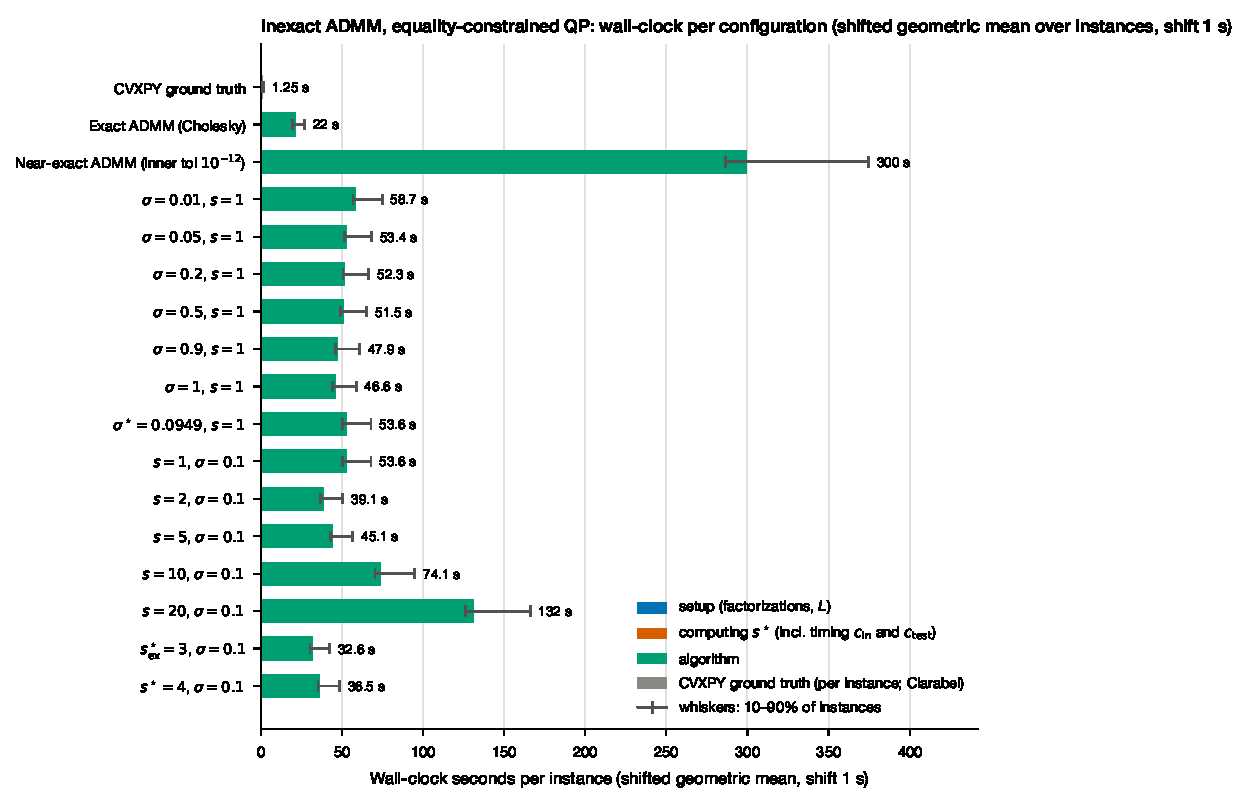
\includegraphics[width=\textwidth]{../results/numerical_experiments/admm_qp/walltime_sgm.pdf}
    \caption{Wall-clock time per configuration on the quadratic programs \Cref{eq:admm-qp} with $n = 2000$ and $m = 600$: the shifted geometric mean over the 100 instances of the setup time, of the time to compute $s^\star$ where it is used (including the timing of $c_{\mathrm{in}}$ and $c_{\mathrm{test}}$), and of the algorithm time, stacked.
    Computing $\sigma^\star$ needs only $\alpha$ and $C_0$ and takes under a millisecond, so its bar has no such segment.
    Whiskers span the 10th to the 90th percentile of the algorithm time, and the top bar is the CVXPY (Clarabel) solve time for scale.
    The configurations are exact ADMM with a Cholesky factorization of $Q + cI$, the near-exact method, the $\sigma$ sweep at $s = 1$ (including $\sigma^\star$), and the $s$ sweep at $\sigma = 0.1$ (including $s^\star$).
    Every configuration that uses GMRES is slower than the factorization, and the inexact ones are faster than the near-exact method.}\label{fig:admm-qp-wall-clock-times}
\end{figure}

The convergence behavior of the outer iterates in \Cref{fig:admm-qp-outer-convergence} is comparable across all configurations; \Cref{fig:admm-qp-outer-convergence-zoom} in \Cref{sec:additional-admm} magnifies its outer-iteration panels.
However, solving the subproblem to extremely high absolute accuracy (in this case, $10^{-12}$) is unnecessary and often detrimental.

\begin{figure}
    \centering
    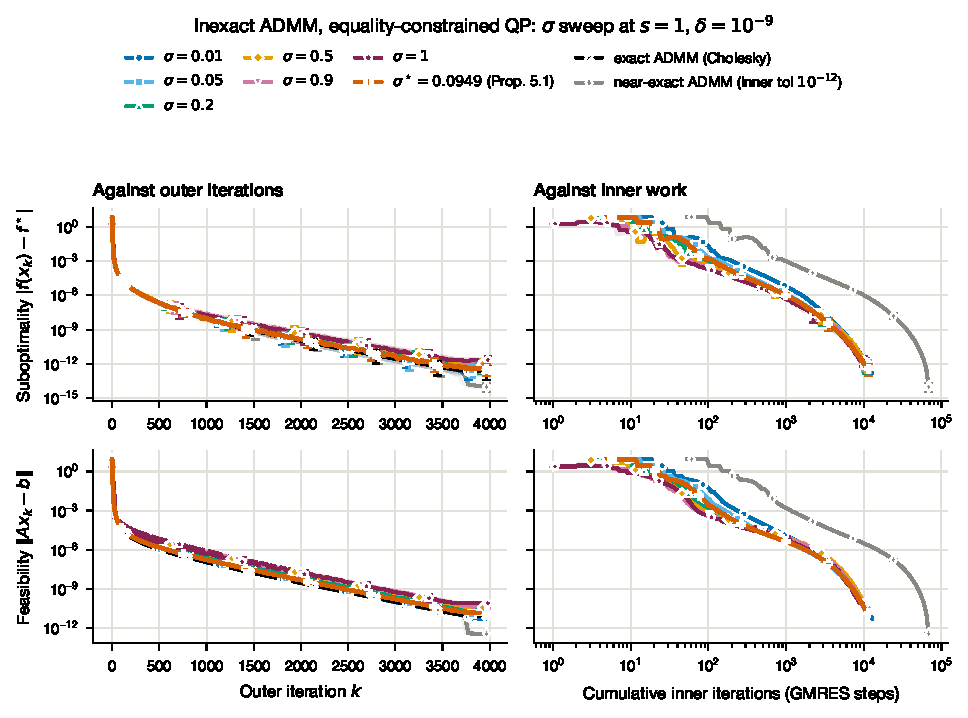
\includegraphics[width=\textwidth]{../results/numerical_experiments/admm_qp/convergence_sigma.pdf}
    \caption{Convergence of \DIFdelbegin \DIFdel{\Cref{alg:inexact-admm} }\DIFdelend \DIFaddbegin \DIFadd{the partially inexact ADMM method described in \Cref{sec:numerical-experiments-admm} }\DIFaddend on the quadratic programs \Cref{eq:admm-qp} for the $\sigma$ sweep at $s = 1$, for $\sigma^\star$, for the near-exact method, and for exact ADMM: suboptimality $|f(x_k) - f^\star|$ (top) and primal feasibility $\norm{Ax_k - b}$ (bottom) against outer iterations (left) and against cumulative GMRES iterations (right).
    Lines are medians over the 100 instances, bands interquartile ranges, and whiskers the 10th to the 90th percentiles; exact ADMM has no inner iterations and appears against outer iterations only.
    The outer-iteration curves are comparable across configurations, while the more inexact ones need the fewest GMRES iterations.}\label{fig:admm-qp-outer-convergence}
\end{figure}

The magnified view in \Cref{fig:admm-qp-outer-convergence-zoom} confirms that the convergence metrics are nearly indistinguishable, and in fact the more inexact configurations perform \emph{better} than the exact ones.
The inexact configurations outperform the theory, which is generally conservative.

As in the previous section, we compare the modeled cost of different choices of $s$ to the actual measured cost.
Numerically solving for a more precise $s^\star$ yields a better result, both theoretically and empirically, as seen in \Cref{fig:admm-qp-optimal-b-star-model}.
The cost of computing $s^\star$, including the timing of $c_{\mathrm{in}}$ and $c_{\mathrm{test}}$, forms the middle segment of the bars that use it, but it is negligible compared to the overall cost of the algorithm and is not visible.
Computing $\sigma^\star$ needs only $\alpha$ and $C_0$, so its bar has no such segment.
\begin{figure}
    \centering
    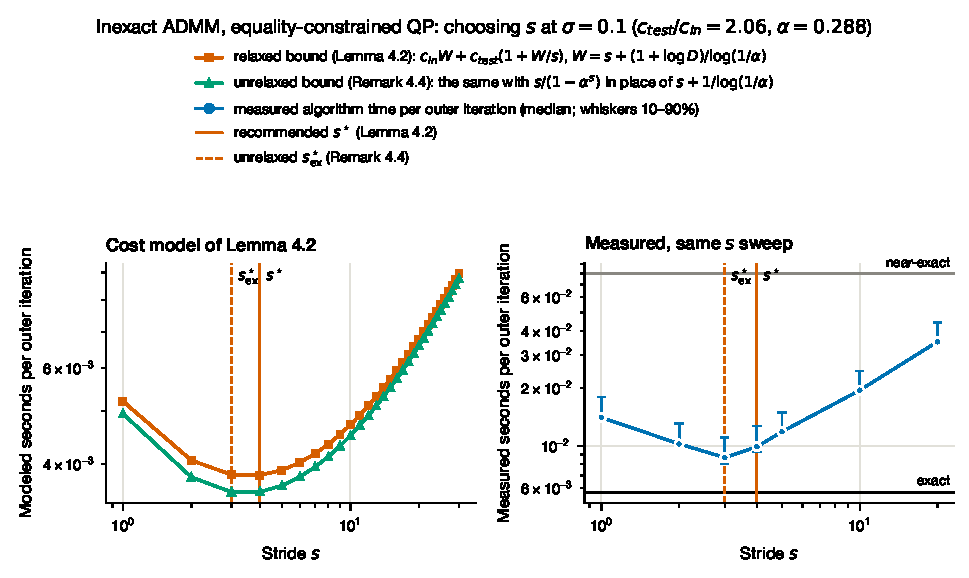
\includegraphics[width=\textwidth]{../results/numerical_experiments/admm_qp/bstar_model.pdf}
    \caption{Choosing the stride on the quadratic programs.
    Left, the modeled seconds per outer iteration as a function of $s$ from \Cref{lem:check-frequency-s-star} (relaxed bound) and from \Cref{rem:b-star-remark} (unrelaxed bound), with their integer minimizers marked; right, the measured seconds per outer iteration of the $s$ sweep at $\sigma = 0.1$ (median over the 100 instances; whiskers from the 10th to the 90th percentile), with the levels of exact ADMM and of the near-exact method as horizontal lines.
    The minimizer of the unrelaxed bound is the better choice, both in the model and in the measurement.}\label{fig:admm-qp-optimal-b-star-model}
\end{figure}

\subsection{Rotation Operator}\label{sec:numerical-experiments-rotation}
We first check the one-step decrease of \Cref{lem:one-step-decrease-inequality} on the two-dimensional Huber instance, and then on an operator for which the lemma is tight for exact steps.
On the two-dimensional Huber instance of \Cref{fig:ppm-huber-trajectories}, the decrease of $\norm{w_k - x^\star}^2$ at each accepted update is well above the amount that \Cref{lem:one-step-decrease-inequality} guarantees for every $\sigma$ (\Cref{fig:huber-fejer-ratio}).
The median over the accepted updates is between $1.77$ and $2.58$ times $\norm{\gamma z_k}^2$ for every $\sigma$ shown, including $\sigma^\star$, against a guarantee of $\frac{1-\sigma}{1+\sigma}$, so the factor $\frac{1+\sigma}{1-\sigma}$ of \Cref{thm:convergence-guarantee} is not reflected in the decrease per accepted step.
To show that this factor is not an artifact of the analysis, we repeat the experiment in two dimensions on the linear operator $\Bcal(x) = U(x-x^\star)$, where $U=\begin{bmatrix}
    0 & -1 \\ 1 & 0
\end{bmatrix}$ is the rotation by a quarter turn.
The operator $\Bcal$ is monotone (but not a gradient).
The instance has $x^\star$ at distance $5$ from the start $x_0 = 0$, and the runs use the same $\sigma$ sweep as before at $s = 1$, with $\delta = 10^{-9}$ and an inner residual of $10^{-12}$ for the near-exact method.
The exact proximal step $w^+$ satisfies $\norm{w - x^\star}^2 - \norm{w^+ - x^\star}^2 = \norm{w - w^+}^2$\footnote{The critical property here is skew-symmetry of $U$.
One could take any higher-dimensional skew-symmetric matrix to get the same exact decrease equality.} and \Cref{lem:one-step-decrease-inequality} is tight for exact steps.
The inner solver is Richardson iteration on the resolvent residual with the step that minimizes its contraction factor, which satisfies \Cref{assumption:inner-work-contraction} with $C_0 = 1$ and $\alpha = \frac{\gamma^2}{1+\gamma^2} = 0.8$ for $\gamma = 2$.
\Cref{fig:torsion-trajectories} shows the paths and \Cref{fig:torsion-fejer-ratio} the observed decrease against its guarantee; the convergence of the sweep, in the layout of \Cref{fig:ppm-huber-outer-convergence}, is \Cref{fig:torsion-convergence} in \Cref{sec:additional-rotation}.
The near-exact method needs $K_\delta = 26$ outer iterations, $\sigma = 0.5$ needs $62$, $\sigma = 0.9$ needs $48$, and $\sigma = 1$ needs $235$, and the median decrease per $\norm{\gamma z_k}^2$ is $1.00$ for the near-exact method, $1.02$ at $\sigma = 0.01$, $0.41$ at $\sigma = 0.5$, $0.28$ at $\sigma = 0.9$, and $0.047$ at $\sigma = 1$, against guarantees of $1$, $0.98$, $0.33$, $0.053$, and $0$.
\begin{figure}
    \centering
    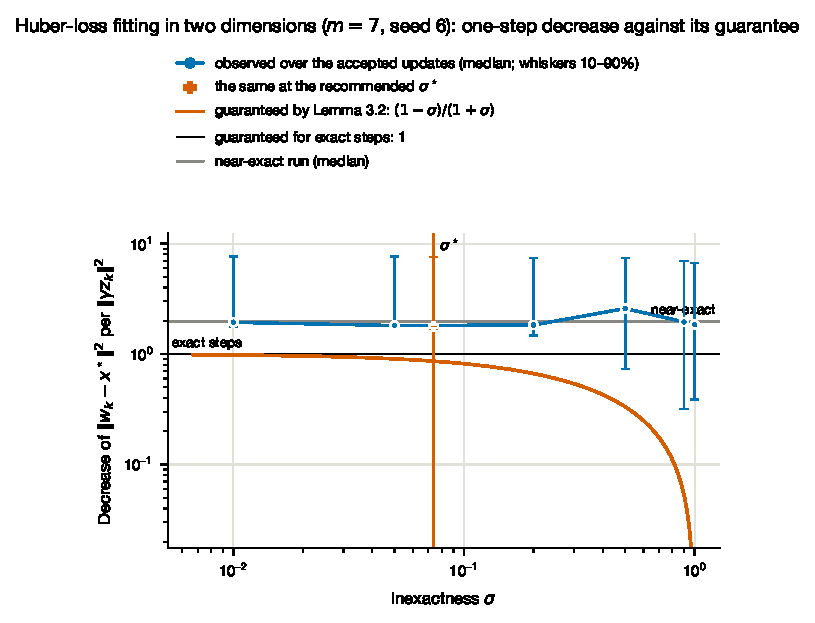
\includegraphics[width=0.7\textwidth]{../results/numerical_experiments/ppm_huber_2d/fejer_ratio.pdf}
    \caption{The decrease of $\norm{w_k - x^\star}^2$ at each accepted update divided by $\norm{\gamma z_k}^2$ on the two-dimensional Huber instance of \Cref{fig:ppm-huber-trajectories}, for the $\sigma$ sweep at $s = 1$ and for $\sigma^\star$ (median over the accepted updates; whiskers from the 10th to the 90th percentile), against the guarantee $\frac{1-\sigma}{1+\sigma}$ of \Cref{lem:one-step-decrease-inequality}, the level $1$ guaranteed for exact steps, and the level observed for the near-exact method.
    The observed decrease stays near the level of exact steps for every $\sigma$.}\label{fig:huber-fejer-ratio}
\end{figure}
\begin{figure}
    \centering
    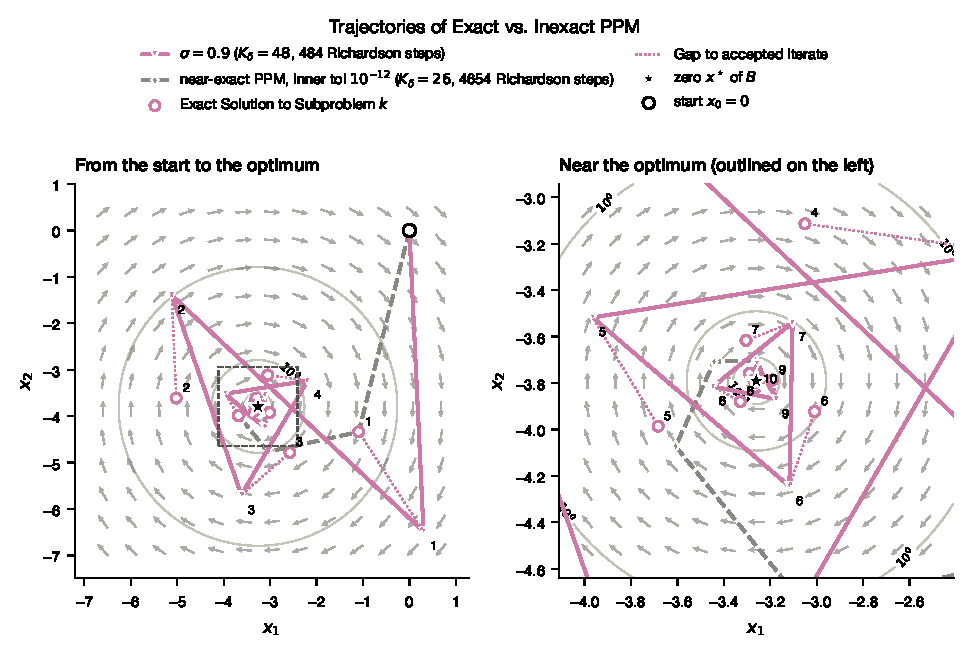
\includegraphics[width=\textwidth]{../results/numerical_experiments/torsion_operator/trajectory_2d_exact.pdf}
    \caption{Accepted iterates of \Cref{alg:stopping-time-algorithm} on the rotation operator $\Bcal(x) = U(x-x^\star)$ for $\sigma = 0.9$ (solid) and for the near-exact method (dashed), at $s = 1$, over contours of $\norm{x - x^\star}$; arrows give the direction of $-\Bcal$, and the right panel magnifies the neighborhood of $x^\star$ outlined on the left.
    Since $\Bcal$ is skew-symmetric, each exact step decreases $\norm{w - x^\star}^2$ by exactly $\norm{w - w^+}^2$, while the inexact iterates wander around $x^\star$ and take 48 outer iterations against 26.}\label{fig:torsion-trajectories}
\end{figure}
\begin{figure}
    \centering
    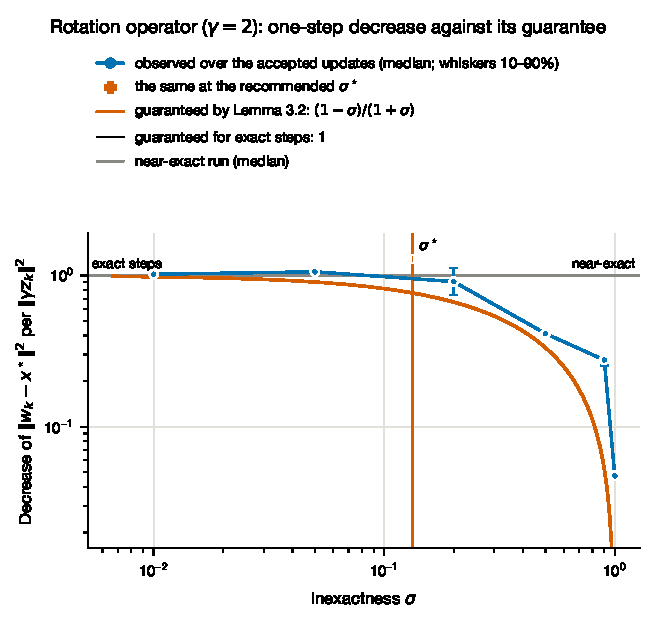
\includegraphics[width=0.7\textwidth]{../results/numerical_experiments/torsion_operator/fejer_ratio.pdf}
    \caption{The decrease of $\norm{w_k - x^\star}^2$ at each accepted update divided by $\norm{\gamma z_k}^2$ on the rotation operator of \Cref{fig:torsion-trajectories}, for the $\sigma$ sweep at $s = 1$ and for $\sigma^\star$ (median over the accepted updates; whiskers from the 10th to the 90th percentile), against the guarantee $\frac{1-\sigma}{1+\sigma}$ of \Cref{lem:one-step-decrease-inequality}, the level $1$ guaranteed for exact steps, and the level observed for the near-exact method.
    The near-exact run attains the exact level, and the inexact runs stay above their guarantee but drop well below the exact level for $\sigma \geq 0.5$.}\label{fig:torsion-fejer-ratio}
\end{figure}